\subsection{Virtual Memory}

In multitasking operating systems, the demand of memory is often greater than the
available physical memory. To solve this problem, virtual memory is introduced.

\textbf{Physical Address} vs \textbf{Logical Address}:
\begin{itemize}
    \item \textbf{Physical Address}: The address used to actually access the physical memory, which can be smaller (e.g. 1 GiB).
    \item \textbf{Logical Address}: The addressing space that a program/process sees, which can be larger. (e.g. 4 GiB if 32-bit)
\end{itemize}

Mapping between logical and physical addresses is done by the \textbf{Memory Management Unit (MMU)}.
Similar to Cache memory, the MMU is based on the principle of locality.
It maps a logical address (of a program) to a physical address (of the memory).

\subsubsection{Paging \& Page Table}

Physical memory is divided into fixed-size blocks called \textbf{frames},
and logical memory is divided into blocks of the same size called \textbf{pages}.

Each process has its own logical address space, hence each process will be divided
into several pages. The OS maintains a \textbf{page table} for each process.

Each page in logical address space has a corresponding page table entry (PTE).
The format of a PTE is roughly:

\begin{table}[H]
    \centering
    \begin{tabular}{cccc}
    1 bit                                & several bits                              & 1 bit                                         & serveral bits                          \\ \hline
    \multicolumn{1}{|c|}{\textbf{V}alid bit} & \multicolumn{1}{c|}{\textbf{P}rotection Bits} & \multicolumn{1}{c|}{\textbf{D}irty Bit} & \multicolumn{1}{c|}{Physical Frame \#} \\ \hline           
    \end{tabular}
\end{table}

\begin{itemize}
    \item \textbf{Valid Bit}: Indicates whether the page is in memory or not.
    \item \textbf{Protection Bits}: Indicate the access rights of the page (read, write, execute, user/kernel access).
    \item \textbf{Dirty Bit}: Indicates whether the page has been modified or not.
    \item \textbf{Physical Frame \#}: The frame number in physical memory where the page is stored.
\end{itemize}

\subsubsection{Demand Paging \& Page Fault}

When a program is loaded, not all its pages are loaded at once. The OS only loads
the pages needed, i.e. on demand, hence the name \textbf{demand paging}.
\textbf{Pros}: fast response since only a few pages are loaded, and less memory usage.
\textbf{Cons}: a lot of page faults until a stable set of pages is loaded.

When the program branches to another instruction on a page that is not in memory,
a \textbf{page fault} occurs. The program will be suspended and the OS will take over
to load the required page, then restart the program.

When the memory is full and no free frames are available, the OS will use different
replacement algorithms to select a frame to be replaced. The algorithms are the same
as those introduced in Section \ref{sec:replacement-algorithms}.

\subsubsection{Address Translation \& TLB}

The logical address has a page \# and an offset. The page number will be used to
look up the page table to find the corresponding physical frame \#. Then, after adding
the offset, the physical address can be obtained and data can be fetched from the memory.

This process involves two memory accesses: page table lookup and data access.
To speed up, a \textbf{Translation Lookaside Buffer (TLB)} is used.
The TLB acts like a cache, which maintains a small number of valid PTEs.
If a PTE is not in TLB, then the page table is consulted.

\begin{figure}[H]
    \centering
    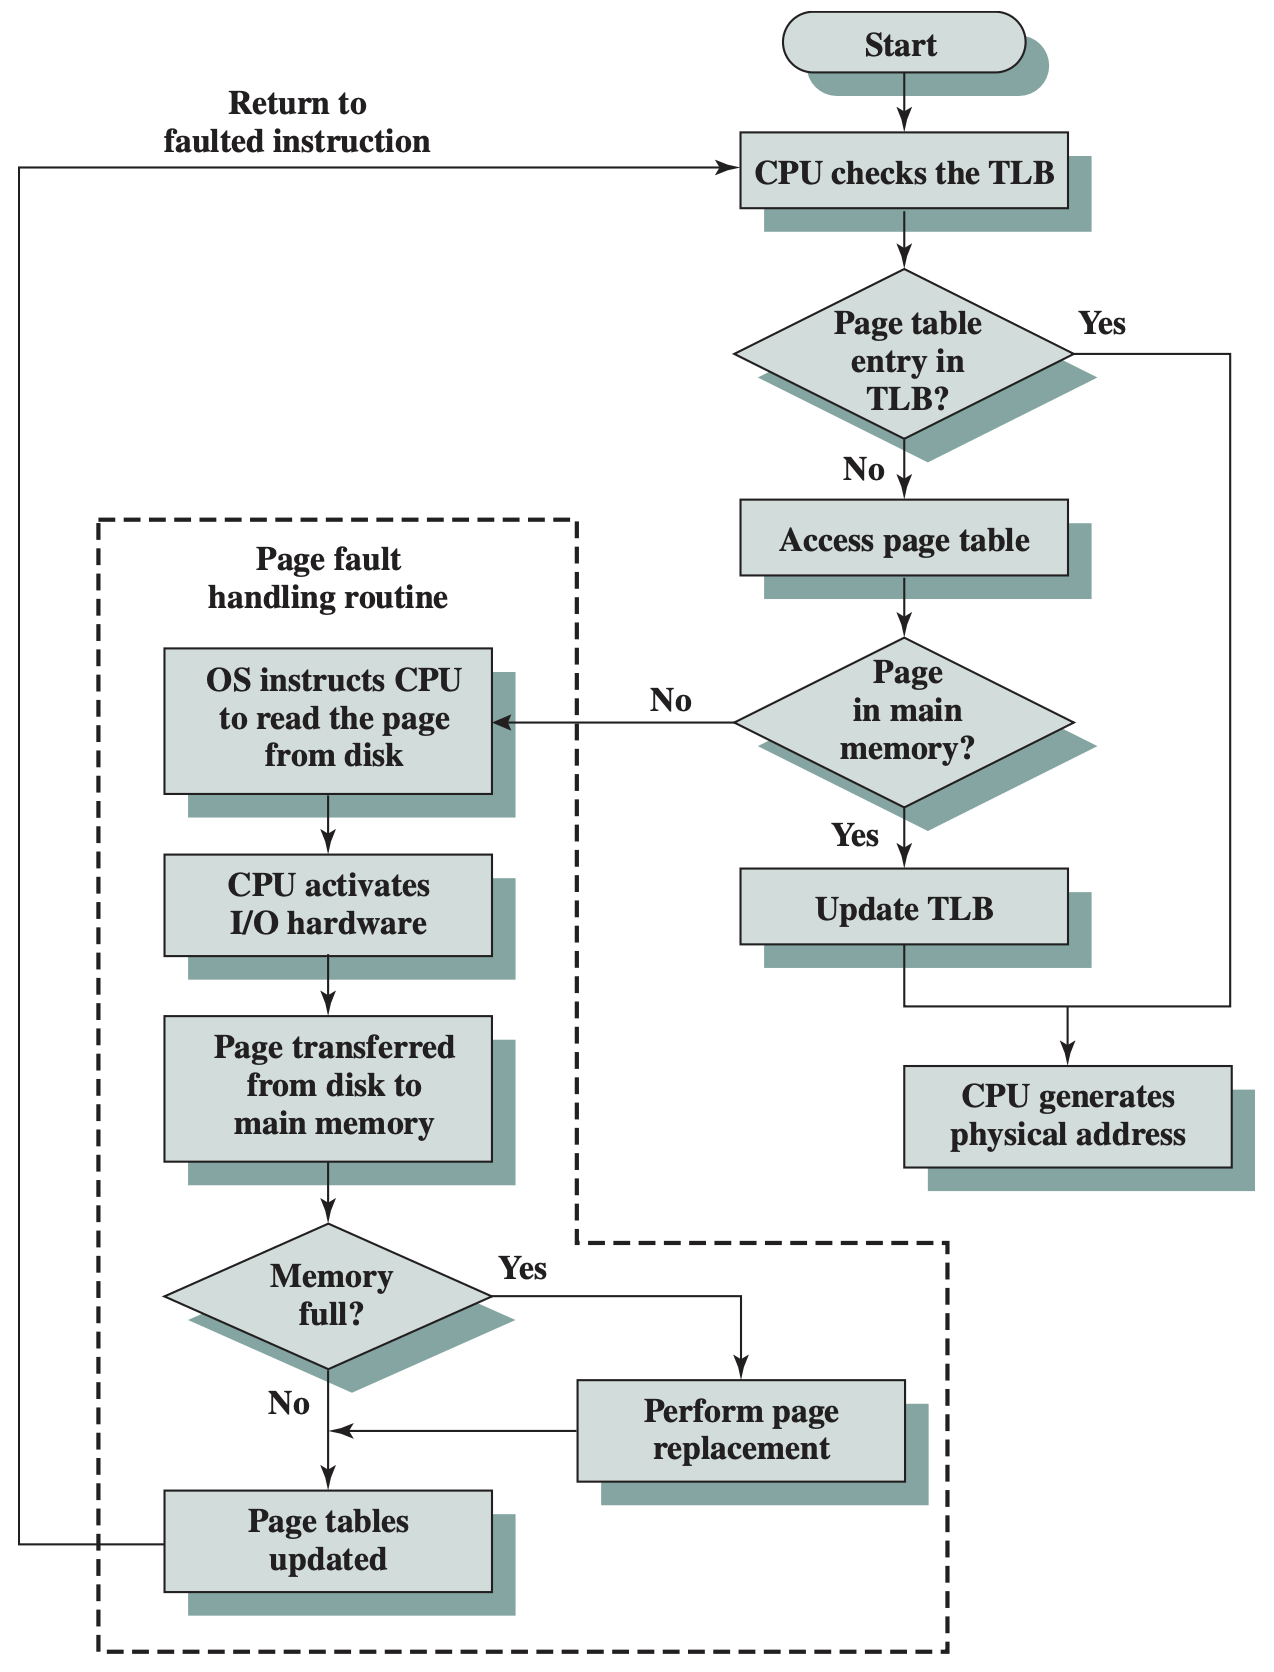
\includegraphics[width=0.6\textwidth]{chaps/memory/virtual-memory/virtual-memory-paging-process.png}
    \caption{Rough process of paging operation}
\end{figure}

\begin{figure}[H]
    \centering
    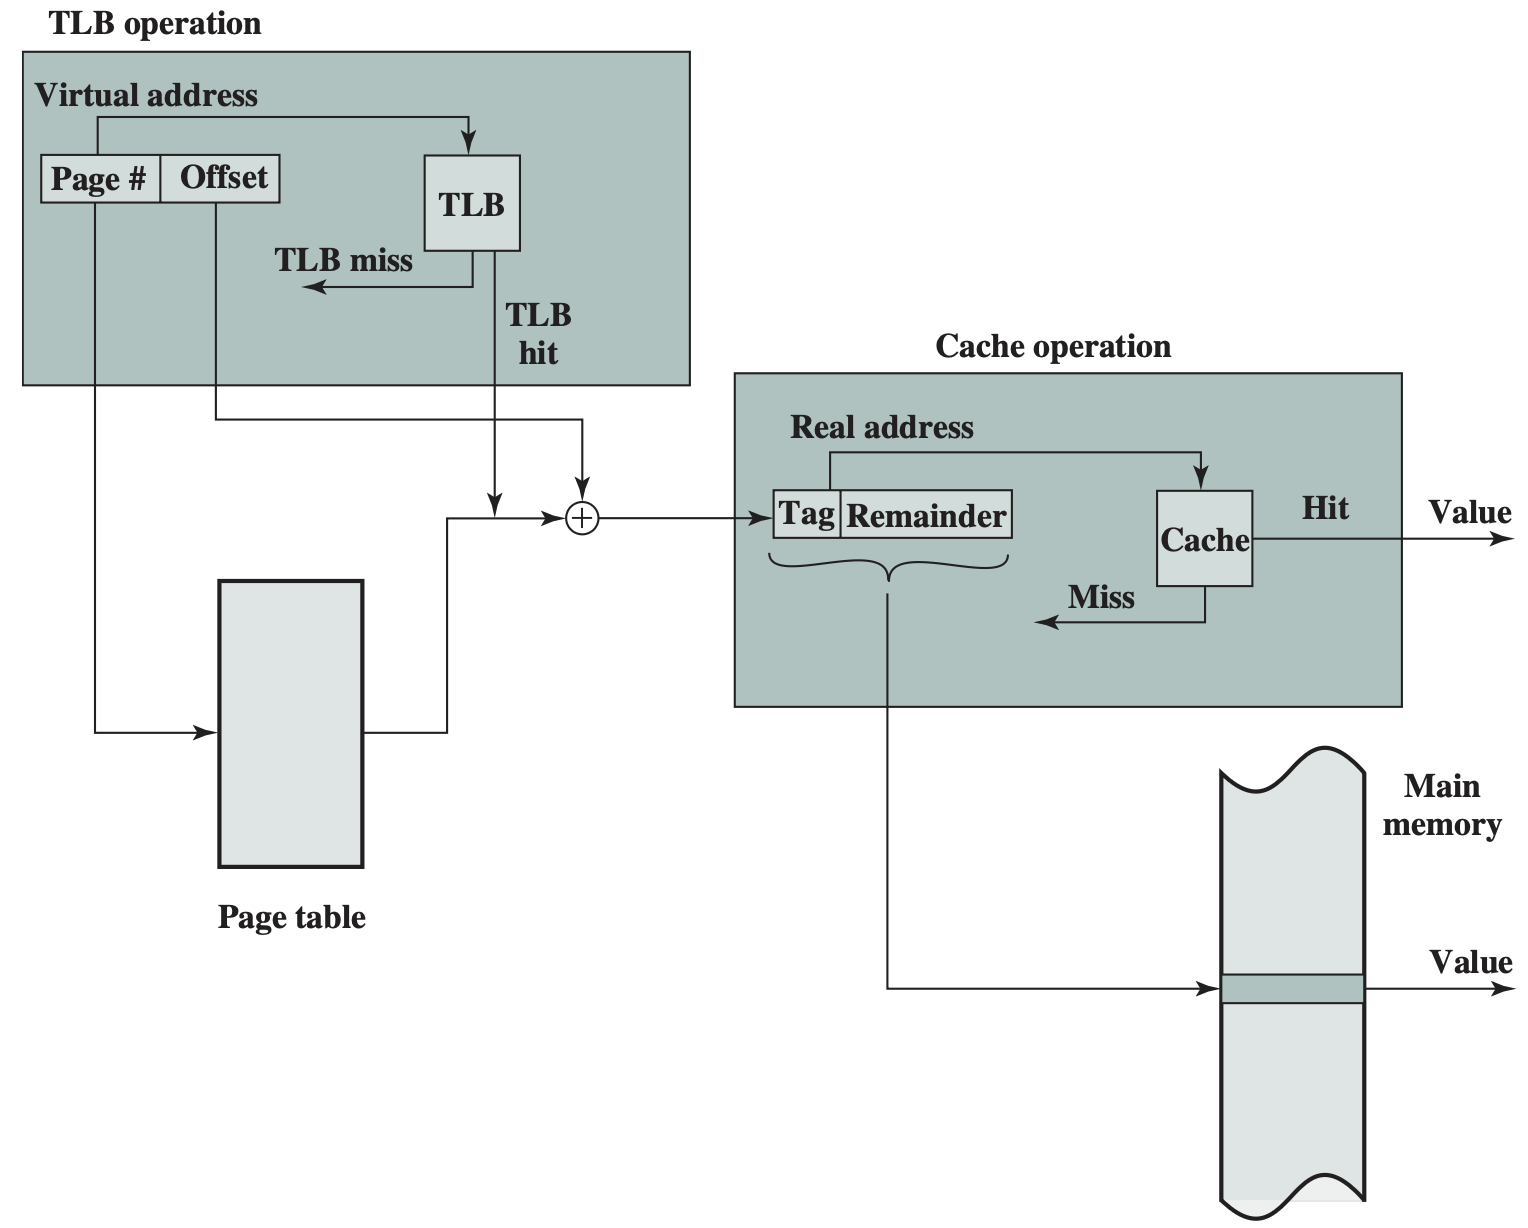
\includegraphics[width=0.65\textwidth]{chaps/memory/virtual-memory/tlb-operation.png}
    \caption{TLB and cache operation}
\end{figure}